This chapter introduces the elements of quantum computing and digital time simulation. First, the qubit as a two-level system and a quantum register as a \textit{multi-qubit} system are presented. After a review of the elements of quantum computing, from single qubit operations to universal quantum computing, digital integration schemes for solving Schrödinger equation are presented. With this background, previous work on simulation of spin and fermionic systems is introduced. Finally, recent techniques fori mplementing hardware efficient two qubit gates are introduced. The present chapter is expected to give a broad overview of the concepts and techniques used in subsequent chapters for implementing a quantum time evolution algorithm for anisotropic Heisenberg-like Hamiltonians.

\section{Quantum circuit model elements}
\label{sec:fundaQC}

  Nowadays, it is familiar to understand information processing tasks in terms of \textit{bits}. A bit is a binary variable that can be said to have either of two states on a set (commonly denoted by $0$, $1$). As a result, a bit is nothing more than a variable $s$ whose value is in the set $\{0,1\}$. In modern computers, such an entity can be encoded physically by means of electric current or voltage. Most operations that can act upon a bit are mappings from one of the possible state values to the other. These corresponds to two fundamental operations: the NOT gate, which flips the bit value, or the IDENTITY gate, whose action is actually inaction.

  In contrast, a quantum bit or \textit{qubit}, corresponds physically to a two-level quantum system, whose Hilbert space can be spanned by a \textit{computational basis set} $\{\ket{0}, \ket{1}\}$. It is reasonable to assume that this basis set is orthonormal

  \begin{equation}
    \braket{s}{s'} = \delta_{ss'} \text{ for } s, s' \in \{0,1\}
    \label{eq:comp-basis}
  \end{equation}

  The canonical representation of a qubit is as a vector in the \textit{Bloch sphere}. This representation maps a generic qubit superposition state

  \begin{align}
    \cos(\frac{\theta}{2}) \ket{0} &  + \mathrm{e}^{\mathrm{i}\phi}\sin(\frac{\theta}{2})\ket{1} \\
    & \theta, \phi \in \mathcal{R}
    \label{eq:qubit-state}
  \end{align}

  To a vector on the unitary 3-sphere

  \begin{equation}
    \hat{\mathbf{n}} = \sin(\theta) \cos(\phi) \hat{\mathbf{x}}  + \sin(\theta) \sin(\phi)\hat{\mathbf{y}} + \cos(\theta) \hat{\mathbf{z}}
    \label{eq:bloch-vector}
  \end{equation}

  In addition to the computational basis, other important states are the \textit{sign basis}

  \begin{gather}
    \ket{+} = \frac{1}{\sqrt{2}}\ket{0} + \frac{1}{\sqrt{2}}\ket{1} \\
    \ket{-} = \frac{1}{\sqrt{2}}\ket{0} - \frac{1}{\sqrt{2}}\ket{1}
    \label{eq:sign-basis}
  \end{gather}

  And the \textit{y basis}

  \begin{gather}
    \ket{+\mathrm{i}} = \frac{1}{\sqrt{2}}\ket{0} + \mathrm{i}\frac{1}{\sqrt{2}}\ket{1} \\
    \ket{-\mathrm{i}} = \frac{1}{\sqrt{2}}\ket{0} - \mathrm{i}\frac{1}{\sqrt{2}}\ket{1}
    \label{eq:phase-basis}
  \end{gather}

  Those states actually lie in the poles of the Bloch sphere, and each pair constitutes a basis for a qubit's Hilbert space that has interesting properties regarding measurement.

  In contrast to classical bits, a quantum bit can be transformed by an infinite number of operations, corresponding to all possible operators defined on its Hilbert space. Of those, two are of huge importance in quantum computing: unitary operators and measurement operators. Unitary operations are used mainly to process quantum information and perform a computation. These are commonly known as \textit{quantum gates}. The fundamental quantum gates are the Pauli operators

  \begin{gather}
    \hat{X} = \ketbra{+}{+} - \ketbra{-}{-} \\
    \hat{Y} = \ketbra{+\mathrm{i}}{+\mathrm{i}} - \ketbra{-\mathrm{i}}{-\mathrm{i}} \\
    \hat{Z} = \ketbra{0}{0} - \ketbra{1}{1}
    \label{eq:pauli-ops}
  \end{gather}
  
  
  For a single qubit, it is known that any unitary operation can be represented as rotation operator of the form

  \begin{gather}
    \hat{R}_{\hat{n}, \theta} = \cos(\frac{\theta}{2}) - \mathrm{i}\sin(\frac{\theta}{2}) \hat{n} \vdot \sigma \\
    \hat{n} \vdot \sigma = n_x \hat{X} + n_y \hat{Y} + n_z \hat{Z} \\
    ||\hat{n}||^2 = 1
  \end{gather}

  In the Bloch sphere representation, quantum gates, therefore, correspond to rotations of the quantum state's associated vector (eq. \ref{eq:bloch-vector}). A quite important rotation is the so called \textit{Hadamard gate}, whose representation in the computational basis is
  
  \begin{equation}
    \hat{H} = \frac{1}{\sqrt{2}}\begin{bmatrix}
      1 & 1 \\
      1 & -1
    \end{bmatrix}
    \label{eq:hadamard-gate}
  \end{equation}
  
  
  These rotations allow computations, but the actual process of reading the outcome of an algorithm implies measurement. In current digital quantum computing implementations, measurement operators are projectors onto the computational basis

  \begin{gather}
    \hat{P}_0 = \ketbra{0}{0} \\
    \hat{P}_1 = \ketbra{1}{1} 
    \label{eq:measurement-ops}
  \end{gather}

  These operators allow measurement of the expected value of $\hat{Z}$ operator. By performing rotations to the sign and y basis, it is possible to measure expected values of $\hat{X}$ and $\hat{Y}$, respectively. Since Pauli operators span the space of qubit operators, any qubit observable can be measured by applying suitable rotations and forming linear combinations of expected values of Pauli operators.

  \subsection{Quantum registers and multi-qubit gates}

    In general, more than one qubit is needed to perform meaningful computations. A system of several qubits is called \textit{quantum register}. A quantum register's Hilbert space is nothing more than the tensor product space of each of its constituent qubits. Thus, a $N$-qubit register has a $2^N$-dimensional Hilbert space. A basis for this space is built by all possible tensor products of computational basis states for each qubit. This would be the \textit{computational basis} of the register. A member of this set may be denoted by

    \begin{gather}
      \ket{s_{N-1}s_{N-2} \cdots s_0} = \ket{s_{N-1}} \otimes \ket{s_{N-2}}\otimes \cdots \otimes \ket{s_{0}} \\
      s_{N-1}, s_{N-2}, \ldots, s_0 \in \{0,1\}
      \label{eq:multi-qubit-basis}
    \end{gather}

    There may be other basis of interest in quantum computing. For instance, with $N=2$, the so called \textit{Bell basis},

    \begin{gather}
      \ket{\Phi^{+}} = \frac{1}{\sqrt{2}}(\ket{00} + \ket{11})\\
      \ket{\Phi^{-}} = \frac{1}{\sqrt{2}}(\ket{00} - \ket{11})\\
      \ket{\Psi^{+}} = \frac{1}{\sqrt{2}}(\ket{10} + \ket{01})\\
      \ket{\Psi^{=}} = \frac{1}{\sqrt{2}}(\ket{10} - \ket{01})
      \label{eq:BellBasis}
    \end{gather}

    is of capital importance in quantum information theory and quantum communications. It will also prove to be important in this work. Much like single-qubit gates, register gates or multi-qubit gates correspond to unitary operators defined on the register's Hilbert space. An important multi-qubit gate, defined by its action on two qubits is CNOT

    \begin{gather}
      \text{CNOT}\ket{\psi}_t \otimes \ket{1}_c = \big(\hat{X}\ket{\psi}_t\big) \otimes \ket{0}_c\\
      \text{CNOT}\ket{\psi}_t \otimes \ket{0}_c = \ket{\psi}_t \otimes \ket{0}_c
      \label{eq:cnot-gate}
    \end{gather}

    Where the subscript $t$ denotes the \textit{target} qubit, and the subscript $c$, the control qubit. Hence, CNOT corresponds to a controlled-$\hat{X}$ operation. This gate can entangle separable two-qubit states. This is of vital importance for universal quantum computing, and can be readily seen from the definition.

  \subsection{Circuit representation}

    This model of computation can be represented graphically by a \textit{circuit}, in which every wire represents a quantum bit, and a gate corresponds to a unitary operator acting on the register's Hilbert space (possibly a Hilbert subspace). For instance, an algorithm for producing a Bell basis state can be represented as in fig. \ref{fig:bell-pair-circuit}

    \begin{figure}[H]
    \centering
    \begin{quantikz}
        \lstick{$\ket{0}$} & \gate{H} & \ctrl{1} & \qw \\
        \lstick{$\ket{0}$} & \qw      & \targ{}  & \qw
    \end{quantikz}
    \caption{Simple algorithm for producing Bell state $\ket{\Phi^{+}}$}
    \label{fig:bell-pair-circuit}
\end{figure}

    In this circuit representation, the algorithm depicted consists on an application of a hadamard operator to a control qubit, followed by a CNOT operation, to a two qubit register on state $\ket{00}$. In general, quantum gates are represented by boxes, labeled properly by the operation that represent. These boxes cover the subspace over which the corresponding quantum operator acts. For instance, in the case of the algorithm depicted on fig. \ref{fig:bell-pair-circuit}, the Hadamard gate acts on a single-qubit subspace, where the CNOT gate acts on the whole two-qubit register's space. Operations are executed from left to right in a quantum algorithm.

  \subsection{Universal quantum computing}
    
    As was stated before, all quantum gates correspond to unitary operations (or measurements), acting on a quantum register. It is desirable to find a set of elementary quantum gates, that act on a small number of qubits, that can generate all possible unitary operations on an $N$-qubit register. This is the question of universal quantum computing. It can be shown that CNOT and the set of single-qubit unitary operations are enough for producing all possible $N$-qubit register gates \cite{Nielsen}. For instance, it is possible to perform the three-qubit \textit{Controlled CNOT} operation

    \begin{gather}
      \text{CCNOT} \ket{\psi} \otimes \ket{s_t} \otimes \ket{s'_t} = \big(\hat{X}^{s_t s'_t} \ket{\psi}\big) \otimes \ket{s_t} \otimes \ket{s'_t} \\
      s_t, s'_t \in \{0,1\}
      \label{eq:toffoli-definition}
    \end{gather}

    by following algorithm on figure \ref{fig:toffoli-universal}. In general, however, performing arbitrary single-qubit rotations by hardware operations is impractical. This would require a huge control on the physical qubits that is not yet available for all possible architectures \cite{Nielsen}. As a result, most quantum processors available today use a limited set of single-qubit rotations for \textit{approximating} arbitrary rotations.

    \begin{figure}
    \centering
    \begin{quantikz}
        \qw & \ctrl{2} & \qw \\
        \qw & \ctrl{1} & \qw \\
        \qw & \targ{}  & \qw
    \end{quantikz}
    =\begin{quantikz}
        \qw & \qw      & \qw      & \qw              & \ctrl{2} & \qw      & \qw & \qw & \ctrl{2} & \qw & \ctrl{1} & \qw & \ctrl{1} & \gate{T} & \qw \\
        \qw & \qw      & \ctrl{1} & \qw              & \qw      & \qw      & \ctrl{1} & \qw & \qw & \gate{T^\dagger} & \targ{} & \gate{T^\dagger} & \targ{} & \gate{S} & \qw \\
        \qw & \gate{H} & \targ{}  & \gate{T^\dagger} & \targ{}  & \gate{T} & \targ{} & \gate{T^\dagger} & \targ{} & \gate{T} & \gate{H} & \qw & \qw & \qw & \qw
    \end{quantikz}
    \caption{Representation of CCNOT (L. H. S.) gate in terms of single-qubit rotations and CNOT (R. H. S.), according to \cite{Nielsen}. Here $\hat{S} = \sqrt{\hat{Z}}$ and $\hat{T} = \sqrt{\hat{S}}$.}
    \label{fig:toffoli-universal}
\end{figure}

    A commonly used universal set is $\{\hat{H}, \hat{S} = \sqrt{\hat{Z}}, \hat{T} = \sqrt{\hat{S}}\}$. With this set, it is possible to approximate any single qubit rotation to an arbitrary precision, but not exactly, using a finite number of operations. In contrast, IBM Quantum devices use a basis set $\{\hat{S}_x = \sqrt{\hat{X}}, \hat{X}, \hat{R}_{z,\phi} \}$, which can reproduce any single-qubit rotation exactly. As an example, the Hadamard gate can be decomposed as follows

    \begin{equation}
      \hat{H} = \hat{R}_{z,\pi/2} \hat{S}_x \hat{R}_{z,\pi/2}
      \label{eq:hadamard-decomp}
    \end{equation}

    As may be inferred from the two examples above, emulating arbitrary $N$-qubit-register operators can cause some computational overhead, that is an increase in the number of elementary operations required to reproduce a quantum computation. Usually, the basis set depends on the architecture of a quantum processor, and thus, due to current limitations of available hardware, it is important to design a quantum algorithm so that the operations involved can be optimally represented by the universal set associated to the device on which it is expected to be implemented.

    Regarding implementation of two qubit gates, an important advance was made by \cite{BellUniversalCartan}. This work shows that implementation of unitary gates in the group
    
    \begin{equation}
      \hat{U}(\alpha, \beta, \gamma) = \mathrm{e}^{-\mathrm{i}(\alpha\hat{X}\hat{X} + \beta\hat{Y}\hat{Y} + \gamma\hat{Z}\hat{Z})}
      \label{eq:CartanDecomp}
    \end{equation}

    Can be performed using only three CNOT gates. Introducing single qubit operators \cite{RXZPulseEfficient}

    \begin{gather}
      \hat{U}_{mn} = \hat{R}_{z}(m\pi/2)\sqrt{X}\hat{R}_{z}(n\pi/2) \\
      \hat{U}_{1\alpha} = \hat{R}_{z}(\pi/2)\sqrt{X}\hat{R}_{z}(\alpha)
      \label{eq:AuxUnitaryCartan}
    \end{gather}

    The circuit representation of such algorithm can be found on figure \ref{fig:cartan3Cnot}

    \input{circuits/cartanThreeCnot.tex}

  \subsection{Quantum computational advantage}
    
    It is expected that quantum computing paradigms challenge the strong Church-Turing thesis, which claims that the ultimate reference for computational complexity is the probabilistic Turing Machine Model \cite{Nielsen, Strini}. In principle, a quantum processor could solve problems that are thought to be hard for probabilistic Turing Machines. Such problems include simulation of chemical systems \cite{QuantumChem1, QuantumChem2}, and multi-particle quantum systems in general \cite{Nielsen, LloydFermSim, BerryErrorBounds}. Regarding the quantum circuit model of computation, this usually means that the total gate count of a circuit that implements an algorithm that solves a hard problem is bounded asymptotically by a polynomial function in the size of the input \cite{Nielsen, Strini}. In general, however, a more accurate measurement of the complexity of a quantum algorithm is the \textit{circuit depth}, which measures the maximum number of operations a qubit has to undergo to complete a computation. One of the goals of this work is to show that it is possible to simulate arbitrarily large spin systems efficiently using quantum digital algorithms, something impossible with the standard methods of computational quantum physics.

\section{Common Approximation Schemes for Unitary Evolution}
\label{sec:trotter}

  Consider a system of $N$ components, whose Hamiltonian can be expressed as a sum of local Hamiltonians (i. e. that model interaction between at most $C$ components) \cite{Nielsen,LloydNature}

  \begin{equation}
    \hat{H} = \sum_{k = 1}^{L} \hat{H}_k
    \label{eq:SparseHam}
  \end{equation}

  Where $L$ is some polynomial on the number of system components. Such system is said to have local interactions between its constituents. From general quantum theory, its dynamics is governed by the Schrödinger equation
  
  \begin{equation}
    \mathrm{i}\dv{\ket{\psi}}{t} = \hat{H}\ket{\psi} 
    \label{eq:Schrodinger}
  \end{equation}

  Whose solution, for time indenependent Hamiltonians, is

  \begin{equation}
    \ket{\psi(t)} = \mathrm{e}^{-\mathrm{i}\hat{H}t}\ket{\psi(0)}
    \label{eq:schrodSolution}
  \end{equation}
  
  In general, $[\hat{H}_i,\hat{H}_j] \neq 0$, and thus

  \begin{equation}
    \mathrm{e}^{-\mathrm{i}\hat{H}t} \neq \prod_{k = 1}^{L} \mathrm{e}^{-\mathrm{i}\hat{H}_kt}
    \label{eq:CommuteUnit}
  \end{equation}

  Hence, solving Schrödinger equation is a non trivial task. Many systems are described by local interactions, for instance, electrons in a solid material or magnetic moments in a lattice. In several instances, local interaction Hamiltonians are non-commuting, and thus approximation methods are necessary for performing time evolution. In this section, schemes for approximating unitary evolution of a quantum system are discussed.

  \subsection{Trotter Formulas}

  Consider operators $\hat{H}_1$, $\hat{H}_2$, with $[\hat{H}_1,\hat{H}_2] \neq 0$. By definition

  \begin{align}
    \mathrm{e}^{-\mathrm{i}\hat{H}_1 t} & = \sum_{m = 0}^{\infty} \frac{(-\mathrm{i}t)^m}{m!}\hat{H}_1^m \\
    \mathrm{e}^{-\mathrm{i}\hat{H}_2 t} & = \sum_{l = 0}^{\infty} \frac{(-\mathrm{i}t)^l}{l!}\hat{H}_2^l
    \label{eq:ExpSeries}
  \end{align}

  It is readily shown that

  \begin{equation}
    \mathrm{e}^{-\mathrm{i}\hat{H}_1 t}\mathrm{e}^{-\mathrm{i}\hat{H}_2 t} = \sum_{k = 0}^{\infty} \frac{(-\mathrm{i}t)^k}{k!} \Bigg[\sum_{m = 0}^k \binom{k}{m} \hat{H}_1^m \hat{H}_2^{k-m}\Bigg]
    \label{eq:ExpProdExact}
  \end{equation}

  Fon non-commuting operators, it is so that

  \begin{equation}
    \sum_{m = 0}^k \binom{k}{m} \hat{H}_1^m \hat{H}_2^{k-m} = (\hat{H}_1 + \hat{H}_2)^k + f_k(\hat{H}_1,\hat{H}_2)
    \label{eq:BinomialTheorem}
  \end{equation}

  Where $f_k(\hat{H}_1,\hat{H}_2)$ is a function of the commutator of the operators. Since $f_1(\hat{H}_1,\hat{H}_2) = 0$, it is so that

  \begin{equation}
    \mathrm{e}^{-\mathrm{i}\hat{H}_1 t}\mathrm{e}^{-\mathrm{i}\hat{H}_2 t} = \mathrm{e}^{-\mathrm{i}(\hat{H}_1 + \hat{H}_2) t} + \mathcal{O}(t^2)
    \label{eq:O2Approx}
  \end{equation}

  If $|t| \ll 1$, the product of the exponential operators estimate the evolution operator with an error $\mathcal{O}(t^2)$. In the general case, it must be noted that

  \begin{equation}
    \mathrm{e}^{-\mathrm{i}\sum_{k = 0}^L \hat{H}_k t} = \hat{1} + (-\mathrm{i}t)\sum_{k = 0}^L \hat{H}_k + \frac{(-\mathrm{i}t)^2}{2} \Bigg[\sum_{k = 0}^L \hat{H}_k^2 + 2 \sum_{j > k}\hat{H}_k \hat{H}_j\Bigg] + \mathcal{O}(t^3)
    \label{eq:TrotterFormula}
  \end{equation}

  In consequence, a unitary evolution operator with local interactions may be approximated, to quadratic order, by the exponential product

  \begin{equation}
    \mathrm{e}^{-\mathrm{i}\sum_{k = 0}^L \hat{H}_k t} = \prod_{k = 1}^{L} \mathrm{e}^{-\mathrm{i}\hat{H}_kt} + \mathcal{O}(t^2)
    \label{eq:2ndOrderTrotter}
  \end{equation}

  In some instances, quadratic approximations may be enough. In his seminal paper, Lloyd presents this quadratic approximation for simulation of quantum systems with local interaction \cite{LloydNature}. Also, Las Heras et. al. simulate a Hubbard Hamiltonian with up to 4 fermionic modes using second order approximations to unitary evolution \cite{HubbardSimul, HubbardSimulLasHeras}. However, in following sections, higher-order approximation schemes are discussed, based upon equation \ref{eq:TrotterFormula}.

  \subsection{Some Cubic Order Schemes}

  The first cubic order approximation discussed is the so called Baker-Haussdorf formulae \cite{Nielsen}. By series expansion, it can be shown that

  \begin{align*}
    \mathrm{e}^{-\mathrm{i}\hat{H}_1t}\mathrm{e}^{-\mathrm{i}\hat{H}_2t}\mathrm{e}^{-\mathrm{i}[\hat{H}_1,\hat{H}_2]t^2} = & \hat{1} + (-\mathrm{i}t) (\hat{H}_1 + \hat{H}_2) \\
    & + \frac{(-\mathrm{i}t)^2}{2}(\hat{H}_1^2 + \hat{H}_2^2 + \hat{H}_1\hat{H}_2 + \hat{H}_2\hat{H}_1) + \mathcal{O}(t^3) \\
    = & \mathrm{e}^{-\mathrm{i}(\hat{H}_1 + \hat{H}_1)t} + \mathcal{O}(t^3)
    \label{eq:Hausdorf1}
  \end{align*}

  Although useful in case of operators that constitute a Lie algebra, the formulae above may not be enough in other instances. A more general approximation formulae is

  \begin{equation}
    \mathrm{e}^{-\mathrm{i}t\sum_{l = 0}^{L-1}\hat{H}_l} = \Bigg(\prod_{l = 0}^{L-1}\mathrm{e}^{-\mathrm{i}\hat{H}_l\frac{t}{2}}\Bigg)\Bigg(\prod_{l = L-1}^{0}\mathrm{e}^{-\mathrm{i}\hat{H}_l\frac{t}{2}}\Bigg) + \mathcal{O}(t^3)
    \label{eq:Suzuki0}
  \end{equation}

  This can be deduced directly from the identity

  \begin{equation}
    \mathrm{e}^{-\mathrm{i}\sum_{l = 0}^{2L-1} \hat{K}_l t} = \hat{1} + (-\mathrm{i}t)\sum_{l = 0}^{2L-1} \hat{K}_l + \frac{(-\mathrm{i}t)^2}{2} \Bigg[\sum_{l = 0}^{2L-1} \hat{K}_l^2 + 2 \sum_{j > l}\hat{K}_l \hat{K}_j\Bigg] + \mathcal{O}(t^3)
    \label{eq:TrotterFormula1}
  \end{equation}

  With the identifications

  \begin{equation}
    \hat{K}_l = \hat{K}_{2L-1-l} = \frac{\hat{H}_l}{2}
    \label{eq:Identifications}
  \end{equation}

  And the following observations

  \begin{equation}
    \begin{gathered}
      \sum_{l = 0}^{2L-1} \hat{K}_l^2 = \frac{1}{2}\sum_{l = 0}^{L-1} \hat{H}_l^2 \\
      2\sum_{l' > l} \hat{K}_{l} \hat{K}_{l'} = \frac{1}{2}\sum_{l = 0}^{L-1} \hat{H}_l^2 + \sum_{l'> l} \Bigg( \hat{H}_{l} \hat{H}_{l'} + \hat{H}_{l'} \hat{H}_{l}\Bigg)\\
      \Bigg(\sum_{l = 0}^{L-1} \hat{H}_l \Bigg)^2 = \sum_{l = 0}^{L-1} \hat{H}_l^2 + \sum_{l'> l} \Bigg( \hat{H}_{l} \hat{H}_{l'} + \hat{H}_{l'} \hat{H}_{l}\Bigg)\\
    \end{gathered}
  \end{equation}

  \subsection{Suzuki - Trotter Scheme}
  This scheme is a higher order approximation to an evolution operator, that works iteratively on top of the approximation given by equation \ref{eq:Suzuki0}. Define \cite{SuzukiFormula, BerryErrorBounds}

  \begin{equation}
    \hat{S}_2(\lambda) = \prod_{l = 0}^{L-1} \mathrm{e}^{\frac{\lambda}{2}\hat{H}_l} \prod_{l = L-1}^{0} \mathrm{e}^{\frac{\lambda}{2}\hat{H}_l}
    \label{eq:SuzukiInit}
  \end{equation}

  Then, for $k > 1$, the following recursion relation is defined

  \begin{equation}
    \hat{S}_{2k}(\lambda) = [\hat{S}_{2k-2}(p_k\lambda)]^2 \hat{S}_{2k-2}((1 - 4 p_k)\lambda) [\hat{S}_{2k-2}(p_k\lambda)]^2
    \label{eq:SuzukiRecursion}
  \end{equation}

  Where coefficients $p_k$ are defined as

  \begin{equation}
    p_k = \frac{1}{4 - 4^{\frac{1}{2k-1}}}
    \label{eq:pk}
  \end{equation}

  It has been shown by Suzuki that \cite{SuzukiFormula}

  \begin{equation}
    \mathrm{e}^{-\mathrm{i}t \sum_{l = 0}^{L-1} \hat{H}_l} = \hat{S}_{2k}(-\mathrm{i}t) + \mathcal{O}(t^{2k+1})
  \end{equation}

  On \cite{BerryErrorBounds}, Barry et. al. show that Suzuki-Trotter schemes can efficiently simulate sparse Hamiltonians, such as the ones considered in this work. As a matter of fact, they have shown that the number of exponentials ($N_{\text{exp}}$) required to simulate time evolution of a system during a time interval $t > 0$, with error bounded by $\epsilon > 0$, is such that

  \begin{equation}
    N_{\text{exp}} \leq 2L5^{2k}(L\tau)^{1+1/2k}/\epsilon^{1/2k}
  \end{equation}

  Where $\tau = \left\Vert \hat{H} \right\Vert t$, $2k$ is the order of a Suzuki-Trotter iteration, and $\epsilon \leq 1 \leq 2L5^{2k}$. Notice that by choosing a sufficiently high order, a Suzuki-Trotter scheme can emulate time evolution with almost linear complexity in time.

  In most cases, simulation of a quantum system by a digital quantum computer requires mapping its Hilbert space to a $2^M$-dimensional Hilbert space. In that case, the number of qubits required for simulation would be $M$. Clearly, all quantum operators in the simulated system's space should be mapped to operators on an $M$-qubit space, which would then be approximated by a universal set of gates. In the following section, demonstrations of this approach to the study of the Hubbard Model and the Electronic structure problem are introduced.

\section{Time Simulation of Spin 1/2 Models}
\label{sec:hubbard}
  
  This section introduces examples of simulation of Hamiltonians such as

  \begin{equation}
    \hat{H} = \sum_{\langle i,j \rangle} J_{ij}^{(x)} \hat{X}_i \hat{X}_j + J_{ij}^{(Y)} \hat{Y}_i \hat{Y}_j + J_{ij}^{(Z)} \hat{Z}_i \hat{Z}_j + \sum_i h_i^{(X)} \hat{X}_i + h_i^{(Y)} \hat{Y}_i + h_i^{(Z)} \hat{Z}_i
    \label{eq:HeisenbergHamiltonian}
  \end{equation}

  Defined over an arbitrary spin graph, and considering nearest neighbor interaction. Most of them are related to work from Las Heras et. al. \cite{HubbardSimul,HubbardSimulLasHeras} and Y. Salathé \cite{HeisenbergSimulLasHeras}. In this section, the importance of simulating such systems is discussed. Furthermore, the examples considered here are further generalized in following chapters to simulate any system whose Hamiltonian is of the shape of eq. \ref{eq:HeisenbergHamiltonian}, and its limitations are exemplified.

  \subsection{Digital simulation of two-spin models}

  As a first example, simulation of two-spin models carried out by Y. Salathé et. al. \cite{HeisenbergSimulLasHeras} are presented. In their work, a superconducting chip with two trasmon qubits is used to simulate two-spin interaction described by the Hamiltonian

  \begin{equation}
    \hat{H}_{1,2}^{x,y} = \frac{J}{2} \bigg( \hat{X}_1 \hat{X}_2 + \hat{Y}_1 \hat{Y}_2 \bigg)
    \label{eq:fundamentalSlatheGate}
  \end{equation}

  This means that they where able to evolve the qubits' state during time $t$, using microwave pulses on the chip, with unitary dynamics governed by Hamiltonian \ref{eq:fundamentalSlatheGate}. It is easy to see that by performing single qubit rotations, it is possible to emulate more complicated dynamics, for instance, an isotropic XYZ interaction

  \begin{equation}
    \hat{H}_{1,2}^{x,y,z} = J \bigg( \hat{X}_1 \hat{X}_2 + \hat{Y}_1 \hat{Y}_2 + \hat{Z}_1 \hat{Z}_2 \bigg)
    \label{eq:XYZSalathe}
  \end{equation}

  An algorithm for simulating time dynamics under Hamiltonian \ref{eq:XYZSalathe} is presented on fig. \ref{fig:salathe-xyz}. The reported state fidelities of the evolution process are above $82\%$. It must be noted that, since all terms of the Hamiltonian commute, the evolution of the two qubit state is exact, and only limited by hardware. In addition to that, an algorithm for simulating the Ising model with transverse homogeneous magnetic field was proposed (see fig. \ref{fig:salathe-ising}).
  
  \begin{equation}
    \hat{H}_I = J \hat{X}_1 \hat{X}_2 + \frac{B}{2}\bigg(\hat{Z}_1 + \hat{Z}_2 \bigg)
    \label{eq:IsingSlathe}
  \end{equation}

  Notice that this Hamiltonian is composed of local parts that do not commute with one another (spin interaction and field interaction), thus an approximate evolution scheme is needed to simulate time evolution. In their work, Salathé et. al. \cite{HeisenbergSimulLasHeras} used a second order trotterization (see eq. \ref{eq:2ndOrderTrotter}). Furthermore, a noise model was proposed to take into account the fact that decoherence and gate errors limit the expected precision of a trotterization scheme. The results show that the main source of error is the infidelity of the two-qubit gate implementation of the XY interaction (eq. \ref{eq:fundamentalSlatheGate}).

  \subsection{Digital simulation of Hubbard models}

  As a second example, the work of las Heras et. al. is considered\cite{HubbardSimulLasHeras}. The authors simulated instances of the quintessential Hubbard Hamiltonian

  \begin{equation}
    \hat{H}_H = -V \sum_{\langle i,j\rangle} (\hat{b}_i^{\dagger}\hat{b}_j + \hat{b}_j^{\dagger}\hat{b}_i) + U \sum_i \hat{n}_{i\uparrow}\hat{n}_{i\downarrow}
    \label{eq:HubbardHamiltonian}
  \end{equation}

  Where $\hat{b}_i$ represent fermionic-mode annihilation operators (for spin-up or spin-down particles), and $\hat{n}_{i\uparrow},\hat{n}_{i\uparrow}$, fermionic-mode occupation number operators. This was done using the Jordan-Wigner mapping, which transforms fermionic operators to qubit operators. The rule is that each occupation mode is mapped directly to the state of a qubit, so that its state encodes the occupation number of the mode in the computational basis. Fermionic annihilation operators are mapped directly following the rule \cite{Mastersthesis}

  \begin{equation}
    \hat{b}_i = \hat{\sigma}_i^{+} \otimes \Bigg(\bigotimes_{k=0}^{N} \hat{Z}_k \Bigg)
    \label{eq:JWT}
  \end{equation}

  Where it is assumed that a linear indexing of the modes is used, even for different spin values. The authors considered models with up to four modes. In particular, they showed that the mapping of a two-mode Hubbard Hamiltonian like eq. \ref{eq:HubbardHamiltonian} leads to a qubit Hamiltonian

  \begin{equation}
    \hat{H}_H = \frac{V}{2}\big(\hat{X}_1 \hat{X}_2 + \hat{Y}_1 \hat{Y}_2\big) + \frac{U}{4} \big(\hat{Z}_1 \hat{Z}_2 + \hat{Z}_1 + \hat{Z}_2\big)
    \label{eq:TwoModeHubbard}
  \end{equation}

  The authors used a superconducting chip for simulating time dynamics governed by Hamiltonian \ref{eq:TwoModeHubbard}. The quantum algorithm is represented on figure \ref{fig:heras-hubbard}. It was used to simulate time evolution with an initial state
  
  $$
  \ket{\psi_0} = \frac{1}{\sqrt{2}}(\ket{0} + \ket{1}) \otimes \ket{0}
  $$

  With $V=U=1$, for a time $t=5$. The results showed that process errors in the implementation of a Trotter step leads to a linear decrease in state fidelity with the number of steps. This is an important factor to consider when implementing Suzuki-Trotter schemes for simulating time evolution. However, their simulations were able to capture the overall dynamics, obtaining fidelities near $90\%$ with a small number of Trotter steps. Three and four mode anisotropic models were simulated as well, obtaining similar results \cite{HubbardSimulLasHeras}.

  It has been shown by Reiner \cite{Mastersthesis} that a one dimensional Hubbard model (eq. \ref{eq:HubbardHamiltonian}) can be mapped to a qubit Hamiltonian of the type \ref{eq:HeisenbergHamiltonian}, by means of the Jordan Wigner mapping. Thus, by generalizing the quantum algorithms presented on these examples, it is possible to study correlation phenomena on metallic solids efficiently, in contrast to current classical simulation methods \cite{Mastersthesis,HubbardOriginal}. In following chapters,  general routines for simulating evolution under Hamiltonian \ref{eq:HeisenbergHamiltonian} are presented, and quantum time evolution is showcased as a tool for studying magnetic properties of solids. Moreover, a discussion of the influence of decoherence and errors in the implementation is carried out, thus presenting the limitations of Suzuki-Trotter schemes for simulating many-body systems.

  \begin{figure}
    \centering
    \begin{subfigure}[b]{1.0\textwidth}
        \centering
        \caption{}
        \begin{quantikz}
            \lstick[wires=2]{$\ket{\psi(0)}$} & \gate[wires=2]{\mathrm{e}^{-\mathrm{i}\hat{H}_{1,2}^{x,y}t}} & \gate{R_{\hat{x}, -\pi/2}} & \gate[wires=2]{\mathrm{e}^{-\mathrm{i}\hat{H}_{1,2}^{x,y}t}} & \gate{R_{\hat{x}, \pi/2}} & \gate{R_{\hat{y}, -\pi/2}} & \gate[wires=2]{\mathrm{e}^{-\mathrm{i}\hat{H}_{1,2}^{x,y}t}} &  \gate{R_{\hat{y}, \pi/2}} & \qw \rstick[wires=2]{$\ket{\psi(t)}$}\\
             & & \gate{R_{\hat{x}, -\pi/2}} & & \gate{R_{\hat{x}, \pi/2}} & \gate{R_{\hat{y}, -\pi/2}} & & \gate{R_{\hat{y}, \pi/2}} & \qw
        \end{quantikz}
        \label{fig:salathe-xyz}
    \end{subfigure}
    \vfill
    \begin{subfigure}[b]{1.0\textwidth}
        \centering
        \caption{}
        \begin{quantikz}
            \gate{R_{\hat{x}, \pi}} & \gate[wires=2]{\mathrm{e}^{-\mathrm{i}\hat{H}_{1,2}^{x,y}\frac{t}{N}}} & \gate{R_{\hat{x}, -\pi}} & \gate[wires=2]{\mathrm{e}^{-\mathrm{i}\hat{H}_{1,2}^{x,y}\frac{t}{N}}} &  \gate{R_{\hat{z}, \frac{t}{N}}} \\
            \qw & & \qw & & \gate{R_{\hat{z}, \frac{t}{N}}}
        \end{quantikz}
        \label{fig:salathe-ising}
    \end{subfigure}
    \begin{subfigure}[b]{1.0\textwidth}
        \centering
        \caption{}
        \begin{quantikz}
            \gate{R_{\hat{y}, \pi/2}} & \gate[wires=2]{\mathrm{e}^{-i\frac{\phi_{xx}}{2}\hat{Z}\otimes\hat{Z}}} & \gate{R_{\hat{y}, -\pi/2}} & \gate{R_{\hat{x}, -\pi/2}} & \gate[wires=2]{\mathrm{e}^{-i\frac{\phi_{yy}}{2}\hat{Z}\otimes\hat{Z}}} & \gate{R_{\hat{x}, \pi/2}} & \gate[wires=2]{\mathrm{e}^{-i\frac{\phi_{zz}}{2}\hat{Z}\otimes\hat{Z}}} & \gate{R_{\hat{z}, \phi_z}} \\
            \gate{R_{\hat{y}, \pi/2}} & & \gate{R_{\hat{y}, -\pi/2}} & \gate{R_{\hat{x}, -\pi/2}} & & \gate{R_{\hat{x}, \pi/2}} & & \gate{R_{\hat{z}, \phi_z}}
        \end{quantikz}
        \label{fig:heras-hubbard}
    \end{subfigure}
    \caption{(a) Digital quantum algorithm for simulating time dynamics of isotropic XYZ model according to \cite{HeisenbergSimulLasHeras}. Notice that commutation of $\hat{X}_1\hat{X}_2$, $\hat{Y}_1\hat{Y}_2$, and $\hat{Z}_1\hat{Z}_2$ implies that the resulting dynamics is exact up to hardware errors. (b) Trotter step for simulating of the Ising model with a transverse magnetic field. This step is repeated $N$ times to evolve over a time interval $t$ \cite{HeisenbergSimulLasHeras}. (c) Trotter step for simulating a two-mode Hubbard model. Here $\phi_{zz} = \phi_z = Ut/2N$ and $\phi_{xx} = \phi_{yy} = Ut/2N$ \cite{HubbardSimulLasHeras}.}
    \label{fig:salathe-circuits}
\end{figure}

\section{Pulse Efficient Circuit Implementations}
\label{sec:pulseFunda}

  In general, current quantum processors are very sensitive to noise. Undesired (and some uncontrollable) interactions may occur between qubits and the environment, or with control and measurement equipment, that lead to a loss of quantum information and coherence of a device's state \cite{quantumEngineer}. In cases of weakly coupled noise sources, decoherence is modeled by qubit energy relaxation and transverse relaxation. The first is related to ground state decay, or depolarization along the $\hat{z}$ axis of the Bloch sphere. The former, is related to decoherence of superposition states, or depolarization on the plane $\hat{x}-\hat{y}$. Those errors are described by characteristic times $T_1$ and $T_2$, respectively, and an exponential relaxation that follows Bloch-Redfield model \cite{quantumEngineer}. Among other sources of error, quantum devices experience thermal relaxation due to interaction with the environment, charge and magnetic flux fluctuations, and decoherence due to photon number fluctuations in the system \cite{quantumEngineer}. 
  
  IBM Quantum devices have characteristic times of tens of microseconds, while common two-qubit gates have implementation times of hundreds of nanoseconds. As a result, most theorized algorithms are unable to run on current devices, due to decoherence \cite{MajoranaSimulation, RXZPulseEfficient, QuantumChem2, QuantumChem1}. Direct transpilation of standard quantum algorithms to the basis set of a quantum device, such as the Quantum Fourier Transform or Quantum Phase Estimation \cite{Nielsen}, even with optimization techniques, require execution times large enough to exceed the coherence times of the qubits.

  In this section, some techniques for quantum control of superconducting qubits are introduced, as well as novel techniques for efficient hardware implementation of quantum algorithms based on the cross resonance interaction \cite{RXZPulseEfficient, 2016RZXCalibration}. Those techniques aim towards optimal usage of the finite coherence times of superconducting qubits on current quantum devices. The insights here presented are the foundations of the time simulation algorithms discussed in following chapters.

  \subsection{Transmon qubits and single qubit gates}

  IBM Quantum devices consist on a set of coupled superconducting qubits known as transmons \cite{Qiskit, quantumEngineer}. A transmon consists on a Josephson junction shunted by a capacitance. Such devices can be described by the quantum variables of charge ($\hat{Q}$) and magnetic flux ($\hat{\phi}$). This due to the collective motion of Cooper pairs in certain superconducting materials. The effective Hamiltonian of a transmon is \cite{quantumEngineer}

  \begin{equation}
    \hat{H}_T = 4E_C \hat{n} - E_J \cos{\hat{\phi}}
    \label{eq:transmonHamilonian}
  \end{equation}

  Where $\hat{n} = \hat{Q}/2e$ is the reduced charge of the transmon. The constants $E_C$ and $E_J$ represent the capacitive and junction energy, respectively. In the transmon regime, the junction energy is much larger than the capacitive energy, and the Hamiltonian \ref{eq:transmonHamilonian} can be simplified to a Duffing oscillator Hamiltonian \cite{quantumEngineer}. The key insight is that the energy levels of the system are separated by different amounts from their immediate neighboring levels. Hence, engineering techniques can be devised for constraining the transmon to the subspace spanned by its first two levels, where the effective Hamiltonian is simply

  \begin{equation}
    \hat{H}_{efe} = -\frac{\omega_0}{2} \hat{Z}
    \label{eq:qubitHamiltonian}
  \end{equation}

  Single qubit gates are implemented on hardware by a capacitive coupling to a microwave signal generator. The process is known as \textit{Rabi driving}, and is carefully summarized on \cite{quantumEngineer}. The advantage of this approach is that rotations around the $\hat{x}$ and $\hat{y}$ axes of the Bloch sphere can be controlled by the phase, amplitude and frequency of the microwave driving (which usually occurs at the resonance frequency of the transmon). Moreover, it is possible to implement \textit{virtual rotations} around the $\hat{z}$ axis by controlling the phase of the drive as illustrated on \cite{quantumEngineer}. Those gates employ zero execution time, and have maximum fidelity. Given that any single qubit unitary has a decomposition

  \begin{equation}
    \hat{U}(\theta, \phi, \lambda) = \begin{bmatrix}
      \cos{\frac{\theta}{2}} & -\mathrm{e}^{\mathrm{i}\lambda}\sin{\frac{\theta}{2}} \\
      \mathrm{e}^{\mathrm{i}\phi}\sin{\frac{\theta}{2}} & \mathrm{e}^{\mathrm{i}(\phi+\lambda)}\cos{\frac{\theta}{2}}
    \end{bmatrix}= \hat{R}_{z, \phi-\pi/2} \sqrt{X} \hat{R}_{z, \pi-\theta} \sqrt{X} \hat{R}_{z, \lambda-\pi/2} 
    \label{eq:qiskitGateImplement}
  \end{equation}

  It is possible to implement arbitrary single qubit rotations with only two microwave pulses at most. This is very similar to the way IBM Quantum backends implement this type of rotations on hardware \cite{Qiskit}. The main sources of error on digital quantum computation are entangling interactions \cite{HeisenbergSimulLasHeras}. In this section, the fundamental notions regarding two qubit gate implementation and novel advances in recent years are presented.

  \subsection{Cross resonance interaction}

  Transmon qubit pairs usually are coupled to one another by a quantum bus whose frequency is different that the resonance frequency of either qubit \cite{quantumEngineer, 2016RZXCalibration}. In most practical applications, the frequency difference of the two qubits is much larger than the coupling strength to the bus. Mathematical modelling of this system uses a Jaynes-Cummings coupling to the bus electromagnetic modes. The details of the study of circuit QED for modelling qubit-qubit interaction can be found on \cite{2020RZXHamiltonianModels}. In general, entangling operations are performed using so called \textit{cross resonance pulses}, in which a target qubit is driven at the \textit{dressed} \footnote{In this context, \textit{dressed} reference the effective qubit frequencies when projecting the Hamiltonian to the subspace of zero excitations of the quantum bus \cite{2020RZXHamiltonianModels}} resonance frequency of the other. For the purpose of this work, it is sufficient to know that the effective interaction between the qubits can be modelled by the \textbf{cross resonance Hamiltonian} \cite{DuplicatedRXZPulse, 2016RZXCalibration}

  \begin{equation}
    \hat{H}_{CR}(\Omega) = \nu_{ZX} \frac{\hat{Z}_1\hat{X}_2}{2} + \nu_{IZ} \frac{\hat{Z}_2}{2} + \nu_{ZI} \frac{\hat{Z}_1}{2} + \nu_{IX} \frac{\hat{X}_2}{2} + \nu_{ZZ} \frac{\hat{Z}_1\hat{Z}_2}{2}
    \label{eq:CRHamiltonian}
  \end{equation}

  Where 1 denotes the control qubit, 2, the target, and the coefficients depend on the driving pulse amplitude $\Omega$. The cross resonance interaction is used on fixed-frequency transmons to implement entangling gates, specifically, highly calibrated CNOT gates. Ideally, cross resonance interaction would only have a $ZX$ interaction, thus generating a controlled rotation gate

  \begin{equation}
    CR(\theta) = \mathrm{e}^{-\mathrm{i}\frac{\theta}{2}\hat{Z}_1\hat{X}_2}
  \end{equation}

  In that case, it would be possible to implement CNOT gates using the decomposition \cite{quantumEngineer}

  \begin{equation}
    \text{CNOT} = \hat{R}_{z_1, \pi/2} \otimes \hat{R}_{x_2, \pi/2} \cdot CR(\theta)
  \end{equation}

  However, experiments show that, in general, all coefficients on Hamiltonian \ref{eq:CRHamiltonian} are non zero \cite{DuplicatedRXZPulse, 2016RZXCalibration}. As a result, undesired terms must be suppressed so that the evolution Hamiltonian is consistent with the target $ZX$ interaction that generates CNOT gates.

  \subsection{Echoed cross resonance gates}

  The current approach towards implementing high fidelity cross resonance gates is outlined on \cite{DuplicatedRXZPulse}. The key insight is that the coefficients of the diagonal terms in the Hamiltonian \ref{eq:CRHamiltonian} are even functions of the pulse amplitude, while the off-diagonal terms are odd functions of this quantity. As a result, by reversing the sign of the driving pulse amplitude, it is possible to mitigate the undesired diagonal terms by evolving the qubits by the operator

  \begin{equation}
    \hat{U} = \mathrm{e}^{-\mathrm{i}\hat{H}_{CR}^{efe}(\Omega)t} = \mathrm{e}^{-\mathrm{i}\hat{H}_{CR}(\Omega)t} \mathrm{e}^{-\mathrm{i}\hat{X}_1\hat{H}_{CR}(-\Omega)\hat{X}_1t}
    \label{eq:pulseCREvolution}
  \end{equation}

  This scheme leads to an effective interaction Hamiltonian \cite{DuplicatedRXZPulse}

  \begin{equation}
    \hat{H}_{CR}^{efe}(\Omega) = \bar{\nu}_{ZX} \frac{\hat{Z}_1\hat{X}_2}{2} + \bar{\nu_{IZ}} \frac{\hat{Z}_2}{2} + \bar{\nu_{IY}} \frac{\hat{Y}_2}{2}
    \label{eq:effectiveHamiltonian}
  \end{equation}

  Undesired unitary error terms can be mitigated by applying appropriate pulses on the target qubit. The general scheme for implementing cross resonance gates on IBM Quantum systems can be seen on figure \ref{fig:echoedPulseQiskit}. The cross resonance drive is carried out by gaussian square pulses, and the $\hat{X}$ pulses are implemented using a Gaussian drive as discussed before in this section. Mathematical details and experimental demonstrations can be found on \cite{DuplicatedRXZPulse, 2016RZXCalibration}.

  \begin{figure}
    \centering
    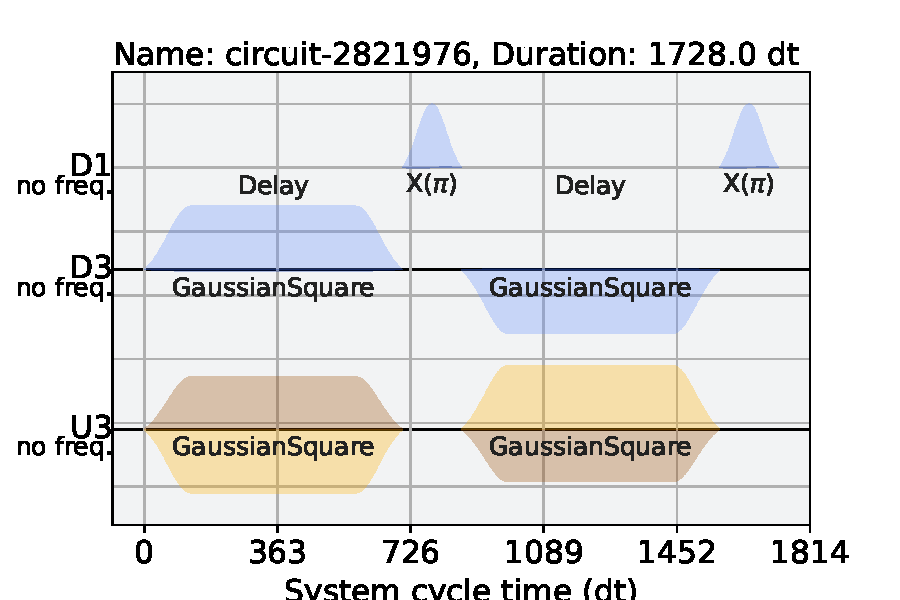
\includegraphics[scale=0.5]{demoEchoedCRPulse.pdf}
    \caption{Echoed cross resonance gate calibration for implementation of CNOT gates in IBM Quantum backends. Control qubit corresponds to index 1, whereas target qubit, to index 3. This figure represents a typical calibration for \textit{ibmq jakarta}.}
    \label{fig:echoedPulseQiskit}
  \end{figure}

  \subsection{Cross-resonance based transpilation of quantum circuits}

  As mentioned before, IBM Quantum exposes a highly calibrated CNOT gates as entangling operations. However, in some instances, CNOT based circuit transpilation to microwave pulse schedules lead to execution times that are impossible to execute with high fidelity on current quantum devices. An example is time simulation of Majorana fermionic systems \cite{MajoranaSimulation}. A key insight towards performing pulse efficient implementation of quantum algorithms is to use the highly calibrated CNOT schedule exposed by IBM Quantum backends to perform cross resonance gates discussed on the previous section \cite{MajoranaSimulation, RXZPulseEfficient}. The details on the gaussian pulse scaling can be found on \cite{MajoranaSimulation}. The idea is to scale the area of the pulses in direct proportion to the angle of rotation of the cross resonance gate. Then, adjust the width, amplitude, and duration of the pulse accordingly. Through Qiskit SDK, it is possible to perform this calibration as discussed in the appendix of \cite{RXZPulseEfficient}.

  As pointed out on \cite{RXZPulseEfficient}, with calibrated cross resonance gates, it is possible to implement two qubit gates of the group

  \begin{equation}
    \hat{U}(\alpha, \beta, \gamma) = \mathrm{e}^{-\mathrm{i}(\alpha\hat{X}\hat{X} + \beta\hat{Y}\hat{Y} + \gamma\hat{Z}\hat{Z})}
    \label{eq:CartanDecomp}
  \end{equation}

  \begin{figure}
    \centering
    \begin{quantikz}
        & \gate{H} & \gate[wires=2]{RZX(\alpha)} & \gate{H} & \gate{S^{\dagger}} & \gate{H} & \gate[wires=2]{RZX(\beta)} & \gate{H} & \gate{S} & \qw    & \gate[wires=2]{RZX(\gamma)} & \qw &\\
        & \qw      &                             & \qw      & \gate{S^{\dagger}} & \qw      &                            & \qw      & \gate{S} & \gate{H} &                                & \gate{H} &
    \end{quantikz}
    \caption{Circuit representation of efficient pulse implementation of unitary operation \ref{eq:CartanDecomp}, according to \cite{RXZPulseEfficient}. Each $RZX$ gate represents a cross resonance interaction with pulse schedule as in figure \ref{fig:echoedPulseQiskit}, with scaling performed as proposed in \cite{MajoranaSimulation}.}
\end{figure}

  As shown on \cite{RXZPulseEfficient} and \cite{MajoranaSimulation}, this type of algorithm transpilation leads to a significant relative error reduction for shorter pulse schedules, allowing time simulation of interesting physical systems. Benchmark test were made in comparison to the three CNOT decomposition depicted on figure \ref{fig:cartan3Cnot}. It was shown experimentally that the relative error can be decreased up to $50\%$ by implementing pulse efficient algorithms on current quantum devices \cite{RXZPulseEfficient}.


